\subsection{The acyclic property for $\nu$-Tamari lattices} 
\label{subsec:nuTamari} 
\nantel{I commented out the original section and input the file "nuTamari"}

We close this section with a theorem that relates our results to the $\nu$-Tamari lattices introduced by L.-F.~Préville-Ratelle and X.~Viennot in~\cite{PrevilleRatelleViennot}. These posets are indexed by a lattice path $\nu$ consisting of a finite number of north~(N) and east~(E) steps, and coincide with the classical Tamari lattices when $\nu=(NE)^n$.

In~\cite{CeballosPadrolSarmiento}, it was shown that the $\nu$-Tamari lattice can be obtained as the increasing flip poset on pipe dreams~$\pipeDreams(\omega_\nu)$ for an explicit permutation $\omega_\nu$ associated to $\nu$. The permutations of the form~$\omega_\nu$ can be easily characterized as follows. We refer to~\cite{CeballosPadrolSarmiento} for details. 

The \defn{Rothe diagram} of a permutation~$\omega$ is the set $\set{(\omega(j),i)}{i<j,\ \omega(i)>\omega(j)}$ in matrix notation.
A permutation $\omega$ is called \defn{dominant} if its Rothe diagram is the Ferrer's diagram of a partition located at the top left corner $(1,1)$. Equivalently, a permutation~$\omega$ is dominant if and only if it is 132-avoiding. 
For a permutation~$\omega = \omega_1 \dots \omega_n \in \fS_n$, we denote by~$0\omega$ the permutation~$0 \omega_1 \dots \omega_n$ of~$\{0, 1, \dots, n\}$, and we consider here pipe dreams with pipes indexed by~$\{0, 1, \dots, n\}$. The Theorem~\ref{prob:nuAcyclicProperty} below states that all pipe dreams with permutation $0 \omega$ are acyclic if and only if $\omega$ is a dominant permutation.
\nantel{modify intro to reflect this?}


From \cref{exm:Tamari1}, we know that this property holds when $\omega=n\dots21$ is the reverse permutation. 
In this case, the increasing flip poset on~$\pipeDreams(0 \omega)$ is the classical Tamari lattice. Removing vertex $0$ from the contact graph of a pipe dream~$ P\in \pipeDreams(0 \omega)$ returns the binary tree corresponding to $P$ (with the leaves removed and the internal nodes labeled from $1$ to $n$).
The edges of the binary tree are oriented going away from the root of the tree.  
See \cref{fig:bijection}. 

Before we start, we need some definition and notation. Given a pipe dream $P$, we say that a crossing is \defn{horizontally connected} if all positions west of it are crossing,
so that the horizontal pipe of the crossing join the west boundary horizontally, without any elbows. Similarly, a crossing is  \defn{vertically connected} if all position north of it are crossing. A \defn{(general) chute move}
is a special increasing flip from a crossing to a northeast contact such that the rectangle defined by these two positions contains only crossing
except in the southeast, northwest and northeast corners (see~\cite[Figure 13]{CeballosPadrolSarmiento}). The following statement appear
in Remark 38 of~\cite{CeballosPadrolSarmiento}, its proof follows from previous result within the cited paper.


\begin{lemma}[\cite{CeballosPadrolSarmiento}]\label{lem:onlychute} 
If $\omega$ is dominant, then any flip of any pipe dream with permutation $0\omega$ is a (general) chute move.
\end{lemma}

The above lemma is very helpful to show our next result.

\begin{lemma}\label{lem:hv_connected} 
If $\omega$ is dominant, then any crossing of any pipe dream with permutation $0\omega$ must be horizontally or vertically connected.
\end{lemma}

\begin{proof}
We proceed by induction on the increasing flip poset of the pipe dreams with $0\omega$ permutation. 
For the greedy pipe dream, where all the crossing are left adjusted, they are all horizontally connected in this case.
We assume the result is true for any crossing in a pipe dream $P$ and show that it still holds  for any crossing of a pipe dream  $Q$ obtained from $P$ by a single flip.
In light of Lemma~\ref{lem:onlychute}, the difference between $P$ and $Q$ must be a single general chute move. As in the picture of the chute portion in $P$ below, 
let $(c,t)$ be the position (row $t$, column $c$) of the crossing that will flip with the contact in position $(d,s)$.
$$	\centerline{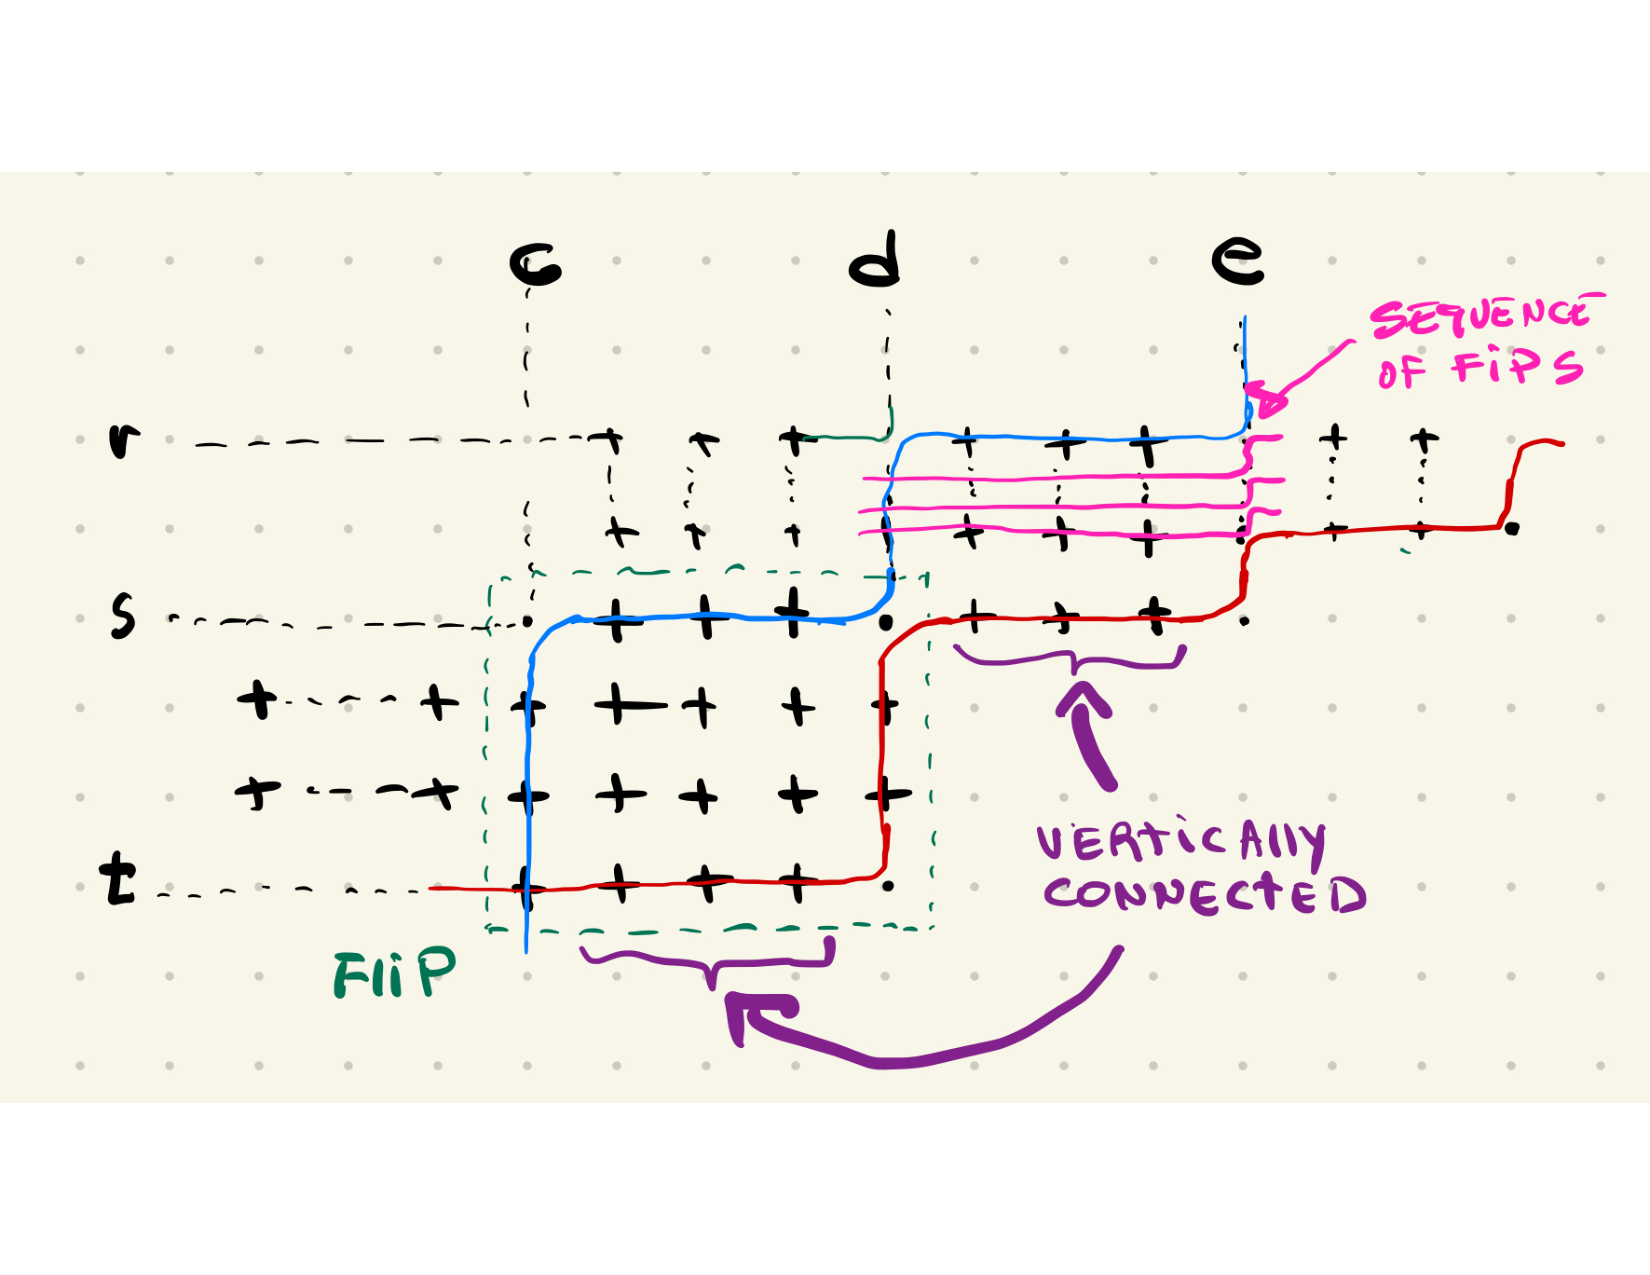
\includegraphics[scale=.2]{chuteofP}}  $$
By assumption, all crossings of  $P$ are either horizontally or vertically connected. Since in position $(c,s)$ there is a contact, any crossing in row $s$ east of column $c$ must
be vertically connected, and by extension all crossing in rows $\le t$ strictly between column $c$ and $d$ are vertically connected.

The pipe dream $Q$ differ from $P$ in only two positions. The crossings of $Q$ are still obviously horizontally or vertically connected is all rows $\ne t$ and all columns $\ne d$.
For row $t$, the remark above shows that in $P$, the crossings strictly between column $c$ and $d$ are vertically connected, so they will still be so in $Q$, resolving all crossings in row $t$
For column $d$, we only need to show that the new crossing in position $(d,s)$ is vertically connected (it cannot be horizontally connected).
We show that we have crossings in column $d$ in all rows $\le s$. Assume for contradiction that there is a contact in row $r<s$ and column $d$.
Let $e$ be the west-most contact east of $d$ in row s. Recall that all crossings in row $s$ strictly between column $d$ and $e$ must be vertically connected (they are east of $c$).

Following Lemma~\ref{lem:horiVertCrossings} and considering $P$, let $i<j$ be the pipes crossing at position $(c,t)$. 
We claim it is not possible to have a crossing in position $(e,r)$, otherwise let $j<k$ be the pipes crossing at position $(e,r)$.
Remark that indeed the pipe $j$ goes through position $(c,t)$ and $(e,r)$, it travel  horizontally west to column d, and south to row s. 
The pipe $k$ at $(e,r)$, going south, cannot be $i$, so it must turn west before row s, travel horizontally and cross $j$ again, a contradiction to $P$ being reduced.
Hence $(e,r)$ must be a contact of $j$ with a pipe $k$.

If the pipe $k=i$, then we have two contacts of $i$ and $j$ in different positions $(d,s)$ and $(e,r)$, this would contradict Lemma~\ref{lem:onlychute}, for the flip of the crossing $(c,t)$
to $(e,r)$ is not a general chute move. If the pipe $k\ne i$, then we remark that, as above, it must cross with $j$ in column $d$ and row $r<r'<s$. We can perform a flip of the crossing
$(d,r')$ with the contact $(e,r)$. This gives us a new pipe dream $P'$ with permutation $0\omega$ similar to $P$ but with an $r'>r$. We repeat the argument in the position $(e,r')$: it cannot be a crossing,
it cannot be a contact with $i$, it must be a contact with a $k'\ne i$. The pipe $k'$ must cross the pipe $j$ in column $d$ and row $r<r'<r''<s$. We can do another flip to get $P''$.
We can only repeat this process finitely many times and after $m<s-r$ steps, we must have a $k^{(m)}=i$ and reach a contradiction. 
Therefor, it is not possible that $P$ has a contact in column $d$ and row $r<s$, and the crossing of $Q$ in position $d,s)$ is vertically connected.
\end{proof}

\nantel{add in acknowledgement that : Lucas Gagnon had a proof of converse in different context}
\begin{theorem}%[The acyclic property for $\nu$-Tamari lattices]
\label{prob:nuAcyclicProperty}
All pipe dreams with permutation $0 \omega$ are acyclic if and only if $\omega$ is a dominant permutation.
\end{theorem}

\begin{proof} For the forward implication, assume that $\omega$ is not dominant. 
Let $P_0$ be the greedy pipe dream of $0\omega$. It has no crossing in row 0, and cannot be a partition starting at row 1.
There must be a row $r>1$ with more crossing than in row $r-1$. 
Considering the rightmost column $c$ of $P$ with a crossing in row $r$,  the pipes $r<k$ are crossing at $(c,r)$, $\omega^{-1}(k)<\omega^{-1}(r)$ and are in contact in position $(c+1,r-1)$.
Let $Q$ be the pipe dream obtained from $P_0$ by the flip of the crossing at $(c,r)$ with the contact at $(c+1,r-1)$.
The contact of $Q$ at $(c,r)$ would gives $r\contactLess{Q} k$. In row $0$ we only have contacts and $\omega^{-1}(k)<\omega^{-1}(r)$, combining this  with Lemma~\ref{lem:rectangle} would give  that 
$k \contactLess{Q} r$, a contradiction, hence $Q$ is not acyclic.

\nantel{Here, I went a bit fast before. Here is a much more detailed version}
For the converse, assume we have a pipe dream that is not acyclic. The contact graph must contain a cycle $i_1 \to i_2\to\cdots\to i_m\to i_1$.
The contact $i_1 \to i_2$ is southeast of $i_1$ and the contact  $i_m\to i_1$ northwest of $i_1$. 
Let $i_k$ be the first time where $i_{k-1}\to i_k$ is a contact southeast of $i_1$ and $i_k \to i_{k+1}$\footnote{with the convention that$k+1$ is $1$ if $k=m$} is a contact northwest of $i_1$.
This implies that the pipe $i_k$ cross $i_1$. Consider the case where $i_1<i_k$, hence $i_k$ is the vertical pipe of the crossing. 
The contact $i_k\to i_{j+1}$ must occur after the crossing of $i_1$ and $i_k$, since it is northwest of $i_1$.
This implies that the crossing of $i_1$ and $i_k$ cannot be vertically connected. 
If $k=2$, then the contact of $i_1\to i_2$ is before the crossing, implying that the crossing of $i_1$ and $i_2$ cannot be horizontally connected. 
The Lemma~\ref{lem:hv_connected} gives that $\omega$ is not dominant in this case.
Assume $k>2$ and assume that the crossing $i_1$ and $i_k$ is horizontally connected. The contact $i_1\to i_2$ is southeast of $i_k$ and the contact $i_{k-1}\to i_k$ is northwest.
Therefor there must be a pipe $i_j$ for $1<j<k$, such that the contact $i_{j-1}\to i_j$ is southeast of both $i_1$ and $i_k$, and the contact $i_{j}\to i_{j+1}$ is southeast of $i_1$ but northwest of $i_j$.
This implies that the pipe $i_j$ and $i_k$ cross southeast of $i_1$ and we must have $i_j<i_k$. The crossing of $i_j$ and $i_k$ cannot be horizontally connected since $i_j$ has a contact west of it.
It cannot be vertically connected since $i_k$ has a contact north of it. Again, Lemma~\ref{lem:hv_connected} gives that $\omega$ is not dominant in this case.

The case where $i_1>i_k$ is very similar, reflecting all arguments. Hence, in all cases, if a pipe dream is not acyclic, then the permutation $\omega$ is not dominant. 
\end{proof}

Applying our Theorem~\ref{thm:pipeDreamQuotient}, we get the following consequence.

\begin{corollary}
If the statement of Open Problem~\ref{prob:nuAcyclicProperty} holds, then the $\nu$-Tamari lattice is a lattice quotient of the interval~$[e,\omega_\nu]$.
\end{corollary}  
